\documentclass{report}
\usepackage{amsmath}
\usepackage{fullpage}
\usepackage{graphicx}
\usepackage{booktabs}
\usepackage{listings}
\usepackage{color}

\definecolor{bwgreen}{rgb}{0, 0.3, 0}
\definecolor{bwblue}{rgb}{0, 0, 0.9}

\usepackage[
	pdfborder={0 0 0 0},
	bookmarks=true,
	colorlinks=true,
	linkcolor=bwblue,
	citecolor=bwgreen
]{hyperref}

\usepackage[all]{hypcap}

\title{Optimization Framework Conceptual Overview}

\lstset{
basicstyle=\ttfamily\footnotesize,
showspaces=false,
showtabs=false,
showstringspaces=false
}

\linespread{1.5}
\setlength{\parindent}{0ex}
\setlength{\parskip}{2ex}
\usepackage{apacite}

\begin{document}

\maketitle

\tableofcontents

\chapter{Conceptual Overview}
Figure \ref{fig:overview} shows a schematic overview of the optimization
framework. There are three distinct layers (user, server and workstation)
in the system. The \textit{user} layer runs the actual optimization process
which will produce tasks that have to be evaluated. These tasks are passed
to the \textit{server} layer which queues them in a task queue. The
\textit{server} acts as a central hub to distribute any tasks it receives
to the available workstations. A \textit{workstation} in turn receives a
single task from the \textit{server} and executes it. When the task has been
evaluated, the result is sent back to the \textit{user} through the
\textit{server} layer. The different layers can run on a single PC, but can
also be placed on different networked PCs. See section \ref{sec:implementation}
for more information on the implementation of the different layers and
communication protocols.

The overall concept of the framework is such that no specific
restrictions are placed on the type of optimization algorithm or the manner
in which a task has to be evaluated. Therefore, the framework can easily be
used for many different and concurrent tasks.

\begin{figure}[h!tb]
	\centering
	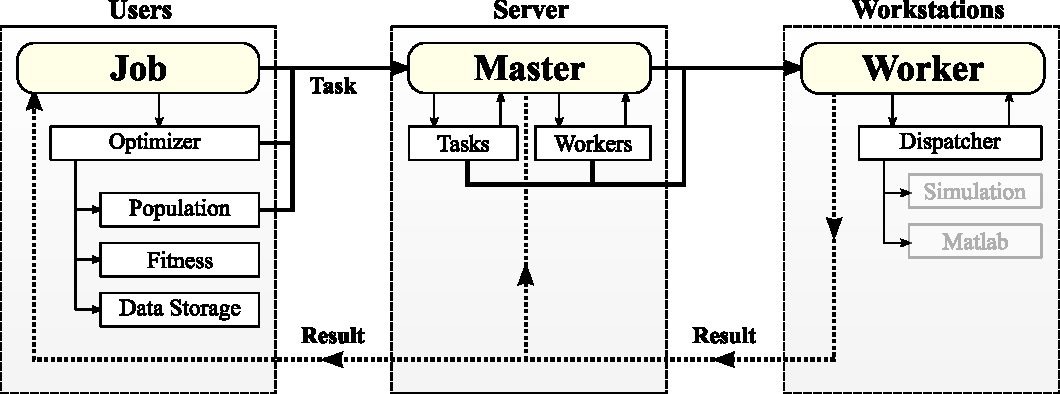
\includegraphics[width=\textwidth]{images/overview}
	\caption{Schematic overview of the optimization framework architecture}
	\label{fig:overview}
\end{figure}

\section{User Layer}
The user layer represents the front-end layer which is run by a user of the
system. This layer is responsible for running the optimization algorithm. The
algorithm produces tasks to be evaluated. As can be seen in figure
\ref{fig:overview}, each optimization, run at the user layer, is encapsulated
in a \textit{Job} process. The job drives the optimization, sends tasks
to the \textit{server} layer, and feeds retrieved results back into the
optimizer.

The optimizer consists of a population (of tasks) that need to
be executed, an optional function which combines a multi-objective fitness evaluation
into a single fitness value, and a data storage to store the results of the
optimization. The optimizer population is a set of tasks that can be executed
independently. For example, in Genetic Algorithms this would be a single
generation of individuals. These represent the set of tasks that can be
distributed at the \textit{server} layer. The fitness function represents
a mathematical expression that can be used to transform multiple objectives
into a single fitness value, used by the optimizer.

A description of the task that is sent to the \textit{server} layer
is given in table \ref{tab:task_message}. Once a task is executed, a result
message as described in table \ref{tab:result_message} is sent back to
the \textit{user} layer.

\begin{table}[h!tb]\caption{Task Message}\label{tab:task_message}\vspace{0.1in}
	\centering

	\begin{tabular}{p{3cm} p{10cm}}
		\toprule
		\textbf{Name} & \textbf{Description} \\
		\midrule
		Id & A unique task identifier \\
		Dispatcher & The dispatcher with which to evaluate the ask \\
		Parameters & A \{\textit{name} $\rightarrow$ \textit{value}\} dictionary of
			         parameters to be evaluated \\
		Settings & A \{\textit{name} $\rightarrow$ \textit{value}\} dictionary of
			       settings to be passed to the dispatcher \\
		\bottomrule
	\end{tabular}
\end{table}

\begin{table}[h!tb]\caption{Result Message}\label{tab:result_message}\vspace{0.1in}
	\centering

	\begin{tabular}{p{3cm} p{10cm}}
		\toprule
		\textbf{Name} & \textbf{Description} \\
		\midrule
		Id & The unique task identifier \\
		Status & Whether the execution was successful or not \\
		Fitness & A \{\textit{name} $\rightarrow$ \textit{value}\} dictionary
		          of fitness values \\
		Data & A \{\textit{name} $\rightarrow$ \textit{value}\} dictionary
		          of additional, custom data to be stored with this task/solution \\
		\bottomrule
	\end{tabular}
\end{table}

\section{Server Layer}
The server layer consists of a single process which acts as a distribution
center for tasks to be evaluated. This layer is used to allow multiple
optimization processes to be run, while sharing the workstation resources that
are currently available. The tasks are scheduled fairly with respect to the estimated
execution time and a task priority. The server automatically discovers new
workstations as they come online through a simple discovery protocol. When
new tasks are received from the \textit{user} layer, it schedules these tasks
(according to their priority) onto a task queue. Whenever a workstation becomes
available, the task is sent to this workstation to be executed. The workstation
then sends the result back to the server, which in turn relays it back to the
\textit{user} layer. Details of the implementation and the used communication
protocols will be discussed in section \ref{sec:implementation}.

\section{Workstation Layer}
The \textit{workstation} layer is responsible for executing a single task, and
sending the result back to the server layer. Each task is received from
the \textit{server} layer with the task information as specified in table
\ref{tab:task_message}. The worker process then resolves a dispatcher process
from the task description that is to be used to evaluate the task. When the
correct dispatcher is located, this dispatcher will be executed with
the task that has to be evaluated. From the dispatcher, the worker will
receive a result in terms of fitness, which it then relays back to the
\textit{server} layer.

\chapter{Implementation}\label{sec:implementation}
This section will give a short overview of the implementation of various parts
of the framework. For more detailed information, see the API documentation.

\section{Communication}
All communication in the framework is implemented using google protobuf. This
is a small, strictly typed, object serialization/deserialization library
developed and released under the BSD open source license by Google. This library
was chosen because it is fast, object oriented, strictly typed and
well maintained. Messages in the framework are mainly sent over TCP/IP, but
UNIX domain sockets are also supported.

\section{Software}
There are two major parts of software developed for the framework. The first
part is the lower level backbone of the framework consisting of the
\textit{server} and \textit{workstation} layers. These layers are implemented in
C++. Common functionality reused in the different components of these layers
is provided in a separate C++ library. The developed applications are:

\begin{itemize}
	\item master (\textit{server} layer): the master distribution process which
	distributes task to workstations
	\item worker (\textit{workstation} layer): the process that accepts tasks
	and executes the appropriate dispatcher
	\item dispatcher (\textit{workstation} layer): the dispatchers that
	evaluate a specific task
\end{itemize}

The \textit{user} layer on the other hand has been implemented in C\# (using
``\textit{mono}'' the open source version of the .NET framework). It consists of a
.NET library containing classes with which optimizers can be easily implemented,
and an application which can run jobs specified using XML. The C\# language
was chosen for this layer because it is easy to learn, modern, powerful,
cross-platform and reduces the time needed to implement new optimization
algorithms.

\section{Security}\label{sec:security}
To support a multi-user environment, the framework can be configured such that
dispatcher processes will be executed under user privileges. When this
functionality is enabled, the \textit{worker} will execute a separate process
that authenticates the task, and if authenticated, executes the dispatcher with
the privileges of the owner of the task. The authentication is based on
a challenge/response mechanisms such that the authentication key of the user
is always send encoded over the network. After successful authentication, the
credentials are confirmed with the permissions to execute the dispatcher
process in question, before dropping to the user credentials. As such, even
if the key would be retrieved, only executables that belong to the user
to whom the key was given can be executed.

\chapter{Applications and Tools}
The following section will describe the applications and tools distributed with
the optimization framework.

\section{optimaster}\label{app:optimaster}
The \verb!optimaster! application represents the server layer of the framework. It
acts as a distribution center for optimization process. You can specify some
options for the \verb!optimaster! using a configuration file in \verb!/etc/optimaster.conf!.
An example configuration file is present in
\verb!/usr/share/optimaster/optimaster.conf.ex!. The available configuration
settings are listed in table \ref{tab:optimaster_configuration}.

\begin{table}[h!tb]\caption{optimaster Configuration}\label{tab:optimaster_configuration}\vspace{0.1in}
	\centering

	\begin{tabular}{p{4cm} p{10cm}}
		\toprule
		\textbf{Name} & \textbf{Description} \\
		\midrule
		\textit{discovery namespace} & the discovery namespace identifies
		                               to which discovery namespace the
		                               \verb!optimaster! belongs. You can use this
		                               namespace to separate different
		                               \verb!optimaster! and \verb!optiworker! processes.
		                               By default, the \verb!optimaster! will set
		                               the namespace to the user name of the
		                               current user. \\
		\textit{discovery address} & the address (IP:port) on which to
		                             broadcast and listen for discovery
		                             messages (usually a multicast address). \\
		\textit{listen address} & the address (IP:port) on which to
		                          listen for incoming optimizer connections. \\
		\bottomrule
	\end{tabular}
\end{table}

\section{optiworker}\label{app:optiworker}
The \verb!optiworker! application represents the workstation layer of the framework. It
receives single tasks from the \verb!optimaster! and executes them according to the
task description. The \verb!optiworker! can run in two modes, \textit{normal} mode
and \textit{token} mode. In \textit{normal} mode, the \verb!optiworker! will launch
dispatcher processes directly and under the same privileges as the \verb!optiworker!
process. In \textit{token} mode, a token system will be used to securely
identify users to which a certain task belongs. In this mode, the
\verb!optirooter! application will be used to launch the dispatcher process.
See section \ref{app:optirooter} for more information.

You can specify some
options for the \verb!optiworker! using a configuration file in \verb!/etc/optiworker.conf!.
An example configuration file is present in
\verb!/usr/share/optiworker/optiworker.conf.ex!. The available configuration
settings are listed in table \ref{tab:optiworker_configuration}.

\begin{table}[h!tb]\caption{optiworker Configuration}\label{tab:optiworker_configuration}\vspace{0.1in}
	\centering

	\begin{tabular}{p{4cm} p{10cm}}
		\toprule
		\textbf{Name} & \textbf{Description} \\
		\midrule
		\textit{discovery namespace} & the discovery namespace identifies
		                               to which discovery namespace the
		                               \verb!optiworker! belongs. \\
		\textit{discovery address} & the address (IP:port) on which to
		                             broadcast and listen for discovery
		                             messages (usually a multicast address). \\
		\textit{use tokens} & whether or not to use the token security system. \\
		\textit{dispatcher priority} & the linux priority level at which to
		                               run the dispatcher processes (see the
		                               `nice` command for more information). \\
		\bottomrule
	\end{tabular}
\end{table}

\section{optirunner}\label{app:optirunner}
The optirunner application is the most important application for the end user.
This application will run the actual optimization process and will be started
by the user. It is possible to use the optimization API to write your own
application that communicates directly with the \verb!optimaster!, but this
should be rarely needed.

The default usage of \verb!optirunner! is by specifying a description of your job
in XML and calling \verb!optirunner! to execute this job. A description of
this XML job representation is given in the next section. Thereafter, a short
explanation of how you can use your own custom optimization algorithms with
optirunner is given.

\subsection{XML description}
The XML description of a job consists of a few distinct sections. The basic
element is \verb!job!:

\vbox{
\begin{lstlisting}[language=xml]
<?xml version="1.0" encoding="UTF-8" ?>

<job name="{NAME}">
  <priority>{PRIORITY}</priority>
  <timeout>{TIMEOUT}</timeout>
  <token>{TOKEN}</token>
  <asynchronous-storage/>
  <!-- Rest -->
</job>
\end{lstlisting}
}

A job should always have a name. The name is used to generate the file name
in which results are written. The \verb!priority!, \verb!timeout!,
\verb!token! and \verb!asynchronous-storage! elements are all \textit{optional}
and specify:

\begin{itemize}
	\item \verb!priority!: the priority level at which you want to run the
	job. This value defaults to 1 if unspecified. Higher priority jobs get
	proportionally more time on the cluster (on average).
	\item \verb!timeout!: timeout indicating the maximum allowed time for
	a task to run. Note that this is measuring \textit{real time} and is
	only used as a safety mechanism for badly behaving dispatchers. You
	almost never have to specify this and is used mostly as a hack to not
	get jobs stuck in never ending tasks.
	\item \verb!token!: an authentication token for the job. See also
	section \ref{sec:tokens} for more information on authentication tokens.
	\item \verb!asynchronous-storage!: when specified, the SQLite database
	is written to disk in asynchronous mode. This can result in significantly
	faster optimizations for tasks that are very shortlived. Note however
	that using asynchronous storage can lead to data loss in case of
	unexpected failures (power outage). The default is to use synchronous
	storage.
\end{itemize}

The remainder of the job description consists of
the \verb!optimizer!, \verb!boundaries!, \verb!parameters! and \verb!dispatcher!
elements defined inside the job element.

The \verb!optimizer! element describes the type of optimization algorithm to
use and any settings that correspond to that particular optimization algorithm.
For example:

\vbox{
\begin{lstlisting}[language=xml]
  <optimizer name="{NAME}">
    <setting name="{SETTING 1}">{VAL}</setting>
    <setting name="{SETTING 2}">{VAL}</setting>
  </optimizer>
\end{lstlisting}
}

The name attribute identifies the optimization algorithm (for example 'pso').
The settings set settings specific to the optimization algorithm. When you
for example use \textit{PSO}, these settings include the maximum allowed
particle velocity and different coefficients used in the algorithm. There are
some settings available for all optimization algorithms, for more information
see section \ref{sec:optimization}.

The \verb!boundaries! element specifies a set of boundary definitions (minimum
and maximum values) which are used in the \verb!parameters! element. An example
boundaries definition:

\vbox{
\begin{lstlisting}[language=xml]
  <optimizer>
    <!-- ... -->
    <boundaries>
      <boundary name="{BOUND 1}" min="{VAL}" max="{VAL}" min-initial="{VAL}" max-initial="{VAL}"/>
      <boundary name="{BOUND 2}" min="{VAL}" max="{VAL}" min-initial="{VAL}" max-initial="{VAL}"/>
    </boundaries>
    <!-- ... -->
  </optimizer>
\end{lstlisting}
}

Each boundary is named, and has a minimum and a maximum value. The name is
used in the parameter definition to reference a specific boundary. The
\verb!min-initial! and \verb!max-initial! attributes are \textit{optional} and
specify respectively the minimum and maximum value to which the initial
population should be initialized (for population based algorithms).

The \verb!parameters! element specifies the set of open parameters to be
optimized. An example definition:

\vbox{
\begin{lstlisting}[language=xml]
  <optimizer>
    <!-- ... -->
    <parameters>
      <parameter name="{PARAMETER 1}" boundary="{BOUNDARY NAME}"/>
      <parameter name="{PARAMETER 2}" boundary="{BOUNDARY NAME}"/>
    </parameters>
    <!-- ... -->
  </optimizer>
\end{lstlisting}
}

Each parameter is named, and specifies by which boundary its value is bound.

In addition to specifying boundaries in a separate section so that they can
be reused, you can also write boundary values in a more concise and simpler
format directly in the parameter specification:

\vbox{
\begin{lstlisting}[language=xml]
  <optimizer>
    <!-- ... -->
    <parameters>
      <parameter name="{PARAM 1}" min="{VAL}" max="{VAL}" min-initial="{VAL}" max-initial="{VAL}"/>
      <parameter name="{PARAM 2}" min="{VAL}" max="{VAL}" min-initial="{VAL}" max-initial="{VAL}"/>
    </parameters>
    <!-- ... -->
  </optimizer>
\end{lstlisting}
}

The optimization framework currently does not support the concept of vectors
or arrays for parameters. Some tasks however are more easily defined using
these concepts (for example, think of weights for a neural network). To
somewhat ease the specification of such repeated parameters, the following
syntax (note the \verb!repeat! attribute) can be used:

\vbox{
\begin{lstlisting}[language=xml]
  <optimizer>
    <!-- ... -->
    <parameters>
      <parameter name="p" repeat="1-10"/>
    </parameters>
    <!-- ... -->
  </optimizer>
\end{lstlisting}
}

This will generate 10 parameters with the names p1 to p10. The specified range
can only contain simple integers (min and max) and these numbers are simply
appended to the specified name. All other attributes (min, max, etc.) can still
be used.

The last element in the optimizer node is the \verb!fitness! element.
This can be used if you have
multiple objectives in your fitness function. By default, if you do not specify
this element, the first fitness value the dispatcher returns is used.
Dispatchers can return multiple fitness values if there are multiple objectives
to be used for optimization. In this case, it can be useful to be able to
define a mathematical expression combining these different values in a single
fitness value. As such, you can adjust the way you combine these different
objectives without having to modify the dispatcher. An example fitness
description:

\vbox{
\begin{lstlisting}[language=xml]
  <optimizer>
    <!-- ... -->
    <fitness>
      <expression>{EXPRESSION}</expression>

      <variable name="{VARIABLE 1}">{EXPRESSION}</variable>
      <variable name="{VARIABLE 2}">{EXPRESSION}</variable>
    </fitness>
    <!-- ... -->
  </optimizer>
\end{lstlisting}
}

The \verb!expression! element in the \verb!fitness! element describes the main
fitness expression to be evaluated. This expression can be a mathematical
expression consistent with most programming languages syntax (operators and
a small set of functions such as log, sin, etc.). The dispatcher will return
a dictionary (name $\rightarrow$ fitness) of fitness values, and you can refer
to such a value by using the name in the expression.

Additionally, you can add any number of variables in the fitness description
containing a mathematical expression. You can refer to these variables from
any expression as well. This can be convenient to specify some weights or
constants which you can later modify easily.

The \verb!dispatcher! element describes the dispatcher and dispatcher settings
to be used to evaluate a solution generated by the optimization algorithm. The
specific settings depend on the type of dispatcher used. An example definition:

\vbox{
\begin{lstlisting}[language=xml]
  <dispatcher name="{NAME}">
    <setting name="{SETTING 1}">{VALUE}</setting>
    <setting name="{SETTING 2}">{VALUE}</setting>
  </dispatcher>
\end{lstlisting}
}

The dispatcher name can be either a simple name, in which case it will be
looked up in the system directory for optimization dispatchers (this is where
system dispatchers such as the webots dispatcher are installed). On the other
hand, you can also specify an absolute path to a dispatcher executable here.

The settings are specific per dispatcher, and are documented separately. Note
that any number of additional settings can be specified here, custom to your
specific job. For instance, using the webots dispatcher, you can retrieve any
additional settings in your webots controller, and configure the simulation
environment accordingly.

\newpage
A full XML job description example:

\begin{lstlisting}[language=xml]
<?xml version="1.0" encoding="utf-8"?>

<job name="example">
  <optimizer name="pso">
    <setting name="population-size">20</setting>
    <setting name="max-iterations">60</setting>
    <setting name="max-velocity">0.6</setting>
    <boundaries>
      <!-- The maximum speed of the e-puck is 1000 -->
      <boundary name="speed" min="100" max="1000"/>
    </boundaries>
    <parameters>
      <parameter name="left" boundary="speed"/>
      <parameter name="right" boundary="speed"/>
    </parameters>
    <fitness>
      <expression>radius - from_origin</expression>
    </fitness>
  </optimizer>
  <dispatcher name="webots">
    <setting name="world">YOUR_PATH/webots/worlds/example.wbt</setting>
    <setting name="mode">batch</setting>
    <setting name="max-time">10</setting>
  </dispatcher>
</job>
\end{lstlisting}

\section{Optimization Algorithms}\label{sec:optimization}
The optimization algorithms currently implemented are:
Particle Swarm Optimization (PSO), Adaptive Diversity Particle Swarm Optimization (ADPSO),
Genetic Algorithms (GA), Simultaneous Perturbation Stochastic Approximation (SPSA)
and Systematic Search (Systematic).

These are available from the \verb!optimizers2-sharp! library. When using
\verb!optirunner!, you can list the available optimization algorithms and
their settings using the \verb!--list! command line option. There are a few
settings common to all optimization algorithms (although some might not apply
to all algorithms). Table \ref{tab:general_settings} lists these settings.

\begin{table}[h!tb]\caption{Optimization Settings}\label{tab:general_settings}\vspace{0.1in}
	\centering

	\begin{tabular}{p{4cm} p{12cm}}
		\toprule
		\textbf{Name} & \textbf{Description} \\
		\midrule
		\textit{population-size} & The population size (applies to
		                           population based methods and has
		                           a special meaning for the
		                           \textit{SPSA} and \textit{Systematic}
		                           algorithms). \\
		\textit{max-iterations} & The maximum number of iterations to
		                          run the optimization (does not apply
		                          to \textit{Systematic}). \\
		\textit{convergence-threshold} & If specified, adds an
		                                 additional stopping criterion
		                                 which is based on measurement
		                                 of convergence. If the
		                                 convergence is below the
		                                 threshold, the optimization
		                                 will be stopped. Convergence
		                                 is measured by:
			\begin{displaymath}
				|\max_{i \in W}{f_i(\mathbf{x})} - \min_{i \in W}{f_i(\mathbf{x})}|
			\end{displaymath}

			Where $W$ is the set of the last
			\textit{convergence-window} iterations and $f_i(\mathbf{x})$
			is the best fitness in iteration $i$. \\
		\textit{convergence-window} & The window (iterations) over which
		                              to measure convergence. \\
		\textit{min-iterations} & The minimum number of iterations to
		                          run before the convergence stopping
		                          criterion is used. \\
		\bottomrule
	\end{tabular}
\end{table}

Each of the available algorithms and their settings will be briefly described.

\subsection{PSO}
The particle swarm optimization is a very elegant, simple and fairly recent
optimization algorithm \cite{kennedy_pso_1995,clerc_pse_2002}. It is
loosely based on the notion of swarm/flocking behavior. The basic algorithm
behind the optimization can be described by:

\begin{eqnarray*}
	v_{ij}(t + 1) & = & \chi (v_{ij}(t) + R_1 \varphi_1 (P_{ij} - x_{ij}(t)) + R_2 \varphi_2 (P_b - x_{ij}(t))) \\
	\chi & = & \dfrac{2k}{|2 - \varphi - \sqrt{\varphi^2 - 4\varphi}|} \\
	\varphi & = & \varphi_1 + \varphi_2 > 4
\end{eqnarray*}

It performs particularly well on real-valued problems with single single
objectives. Table \ref{tab:pso_settings} lists the settings available for this
optimization algorithm.

\begin{table}[h!tb]\caption{PSO Settings}\label{tab:pso_settings}\vspace{0.1in}
	\centering

	\begin{tabular}{p{4cm} p{12cm}}
		\toprule
		\textbf{Name} & \textbf{Description} \\
		\midrule
		\textit{max-velocity} & The maximum particle velocity as a fraction of
		                        the parameter space \\
		\textit{cognitive-factor} & The PSO cognitive factor as described in the
		                            literature ($\varphi_1$) \\
		\textit{social-factor} & The PSO social factor as described in the
		                         literature ($\varphi_2$) \\
		\textit{constriction} & The velocity update constriction as described
		                        in the literature ($\chi$). \\
		\textit{boundary-condition} & The action to take when particles reach
		                              the parameter boundaries (\verb!None!,
		                              \verb!Stick! or \verb!Bounce!). The
		                              default is \verb!Bounce!. \\
		\textit{boundary-damping} & A velocity damping factor when the boundary
		                            condition is \verb!Bounce!. \\
		\bottomrule
	\end{tabular}
\end{table}

\subsection{ADPSO}
Adaptive Diversity Particle Swarm Optimization is a variant of the standard
PSO algorithm that introduces collision detection and particle dispersion
using adaptive, per particle collision radi and adaptive collision reaction
forces \cite{monson_ad_2006}. It is a fairly elegant solution for resolving
some of the deficits of the standard PSO such as premature convergence. It
performs better on multi modal functions than the standard PSO.

The collision radius $c_r$ is defined by:

\begin{eqnarray*}
	c_r & = & \gamma^{b_i} + \gamma^{b_j} r
\end{eqnarray*}

With $\gamma$ an adaptation constant, $b_i$ and $b_j$ the respective number
of times particles $i$ and $j$ have collided until now and $r$ a basic collision
radius. As can easily seen, the collision radius per particle decreases
the more it collides.

When two particles collide, their velocity is reflected and their new position
is calculated by:

\begin{eqnarray*}
	x'_{t + 1} & = & x_t - \gamma^{-b}(x_{t + 1} - x_{t})
\end{eqnarray*}

Thus reflecting the current position around the old position, weighted by
$\gamma^{-b}$. Thus, as the adaptive radius decreases with increased number
of collisions, the bounce distance increases. This allows both good convergence
and escaping of local minima.

Table \ref{tab:adpso_settings} lists the settings available for this optimizer.
ADPSO is an extension of the standard PSO and the PSO settings defined in
table \ref{tab:pso_settings} also apply to this optimization algorithm. For
more information on the available settings, see \citeA{monson_ad_2006}.

\begin{table}[h!tb]\caption{ADPSO Settings}\label{tab:adpso_settings}\vspace{0.1in}
	\centering

	\begin{tabular}{p{4cm} p{12cm}}
		\toprule
		\textbf{Name} & \textbf{Description} \\
		\midrule
		\textit{adaptation-constant} & The adaptation constant ($\gamma$) with regard to the number
		                      of times a particle has collided (0 - 1) \\
		\textit{collision-radius} & The basic collision radius ($r$) as a fraction of the
		                   parameter space \\
		\bottomrule
	\end{tabular}
\end{table}

\newpage

\subsection{SPSA}
Simultaneous Perturbation Stochastic Approximation is an efficient,
popular, stochastic gradient descend method \cite{spall_multivariate_1992}. It
can be defined by:

\begin{eqnarray*}
	\hat{\theta}_{k + 1} & = & \hat{\theta}_k - a_k \hat{g}_k(\hat{\theta}_k) \\
	\hat{g}_{ki}(\hat{\theta}_k) & = & \frac{y(\hat{\theta}_k + c_k \Delta_k) -
	                                         y(\hat{\theta}_k - c_k \Delta_k)}{2 c_k}
\end{eqnarray*}

With $\hat{\theta}_k$ the solution estimation at iteration $k$, $a_k$ a learning
rate, $\hat{g}_k(\hat{\theta}_k)$ the estimation of the gradient at
$\hat{\theta}_k$, $y$ the objective function, $c_k$ a perturbation rate and
$\Delta_k$ the randomized perturbation vector.

The current implementation performs this two-sided perturbation to estimate the
gradient with the perturbation vector $\Delta_k$ drawn from a Bernoulli $\pm$
distribution to satisfy convergence conditions.

Table \ref{tab:spsa_settings} lists the settings available for this optimizer.

\begin{table}[h!tb]\caption{SPSA Settings}\label{tab:spsa_settings}\vspace{0.1in}
	\centering

	\begin{tabular}{p{4cm} p{12cm}}
		\toprule
		\textbf{Name} & \textbf{Description} \\
		\midrule
		\textit{learning-rate} & The learning rate $a_k$ used to update the
		                         new solution according to the current gradient
		                         estimation. You can use a mathematical
		                         expression for this setting and use the
		                         variable $k$ to indicate the current iteration
		                         number \\
		\textit{perturbation-rate} & The rate $c_k$ with which to perturbate the
		                             solution to estimate the gradient. You
		                             can use a mathematical expression for this
		                             setting and use the variable $k$ to
		                             indicate the current iteration number \\
		\textit{epsilon} & The normalized maximum parameter step size. You
		                    can use a mathematical expression for this
		                    setting and use the variable $k$ to indicate the
		                    current iteration number \\
		\textit{boundary-condition} & Indicates how parameter boundaries
		                              should be handled. There are three
		                              possible settings: \textit{None}
		                              (does not contrain the parameter
		                              space), \textit{StickResult} (only
		                              constrains the actual solution to
		                              be within the parameter boundaries)
		                              and \textit{StickAll} (constrains
		                              both the actual position and the
		                              perturbed solutions to be within
		                              the parameter boundaries). \\
		\bottomrule
	\end{tabular}
\end{table}

\newpage

\subsection{GA}
This optimizer implements the well known standard implementation of
Genetic Algorithms. Table \ref{tab:ga_settings} lists the settings available
for this optimizer.

\begin{table}[h!tb]\caption{GA Settings}\label{tab:ga_settings}\vspace{0.1in}
	\centering

	\begin{tabular}{p{4cm} p{12cm}}
		\toprule
		\textbf{Name} & \textbf{Description} \\
		\midrule
		\textit{selection} & The type of selection mechanism to use to make
		                     new populations. Available are ``Tournament'' and
		                     ``RouletteWheel''. Tournament selection is the
		                     default \\
		\textit{tournament-size} & The number of individuals to use for
		                           tournament selection. Applies only when
		                           selection is ``Tournament'' \\
		\textit{tournament-probability} & Probability with which an individual
		                                  is selected from a tournament:
		                                  $p (1 - p)^i$ with $i$ the individual
		                                  order. You can use a mathematical
		                                  expression for this setting and use
		                                  the variable $k$ to indicate the
		                                  current iteration number. Applies only
		                                  when selection is ``Tournament'' \\
		\textit{mutation-probability} & The probability with which to mutate an
		                                individual. You can use a mathematical
		                                expression for this setting and use
		                                the variable $k$ to indicate the
		                                current iteration number \\
		\textit{mutation-rate} & The maximum amount of mutation as a fraction
		                         of the parameter space. You can use a mathematical
		                         expression for this setting and use
		                         the variable $k$ to indicate the
		                         current iteration number \\
		\textit{crossover-probability} & The probability with which to use
		                                 cross-over to create a new individual
		                                 from two selected parent individuals.
		                                 You can use a mathematical
		                                 expression for this setting and use
		                                 the variable $k$ to indicate the
		                                 current iteration number \\
		\bottomrule
	\end{tabular}
\end{table}

The GA implementation supports both real valued as discrete valued parameters.

\subsection{Systematic Search}
The systematic search optimizer is not an optimization algorithm, but instead
performs a systematic parameter search on a range of parameters. This is an
example of how the distribution of tasks by the framework can be used for
purposes other than strictly optimizations.

This optimizer extends the job XML description so that you can specify the
range for each parameter to explore systematically instead of just the upper
and lower boundary as done normally. An example description:

\begin{lstlisting}[language=xml]
  <optimizer>
    <!-- ... -->
    <parameters>
      <parameter name="{NAME 1}" min="{MIN}" max="{MAX}" step="{STEP}"/>
      <parameter name="{NAME 2}" min="{MIN}" max="{MAX}" steps="{STEPS}"/>
    </parameters>
  </optimizer>
\end{lstlisting}

You can specify ranges in two different ways, either by specifying the step
size explicitly (first parameter in the example) or by specifying the number of
steps that should be explored (second parameter in the example). In the second case
the step size will be automatically calculated.

There are no additional settings for the systematic search. The default
\textit{population-size} setting determines the batch size in which
solutions are sent to the \verb!optimaster!. You should set this to a
sensible value (around 200/300 or something).

\section{optirooter}\label{app:optirooter}
The \verb!optirooter! application can be used by the \verb!optiworker! to execute dispatcher
process under the privileges of the user owning the actual task being executed.
This application will use the token server to identify which user the current
task belongs to. When used, the \verb!optirooter! will receive a challenge key from
the token server, which is relays back to the \verb!optiworker!, \verb!optimaster! and
finally optirunner application. The optirunner will then encrypt this challenge
with a unique token generated by the token server before starting the job. This
is send back to the \verb!optirooter! which verifies to which user this encrypted
token belongs. On success, it will drop privileges to this user, and execute
the dispatcher process. Before dropping privileges, the dispatcher is
verified to be either a system installed dispatcher, or a dispatcher owned
by the user (and located in the users' home directory) to which it will
drop privileges. Note that the \verb!optirooter! application has to be setuid and
owned by root.

\section{optiextractor}\label{app:optiextractor}
The optiextractor application can be used to inspect a results database. You
can use it to view the settings, parameters and boundaries of a specific
job. It also features the possibility to automatically replay a specific
solution found during optimization. This is particularly useful in conjunction
with for instance webots, to quickly view a particular solution.

You can export the database to a matlab file which can be directly loaded
into matlab. Either use the \textit{Export} command from the menu, or use the
\verb!--export! command line argument.

\section{opticommand}\label{app:opticommand}
The opticommand application can be used to inspect the optimaster, displaying
which jobs it is running, and how far along the jobs are. To use it, simply
launch \verb!opticommand! from the command line. For a list of commands, type
\verb!help!. If you want to connect to a remote master, use
\verb!opticommand -m <hostname>[:port]!.

\section{Dispatchers}
There are a few dispatchers available by default. This section will shortly
describe these dispatchers.

\subsection{Webots}
The webots dispatcher can be used to evaluate solutions in webots. The
dispatcher will launch a webots process for each task it receives and runs
the world file specified in the dispatcher settings. In your controller, you
can make use of the optimization::Webots class (see liboptimization API
documentation for more information) to extract the task description and setup
your controller accordingly. The specific dispatcher settings for the webots
dispatcher are listed in table \ref{tab:webots_settings}.

Sometimes it might be necessary to change the world file according to your task
description. To this end, a special setting is available (\textit{worldBuilderPath})
which specifies an executable that will dynamically build the webots world
file to use instead of specifying it in the \textit{world} setting. The
world builder executable will be executed before the webots process is executed
and will receive the task description on \verb!standard in!
(just as for the dispatcher). It should then generate the world file and
write the path to this world file on \verb!standard out!. It can be useful
to use the optimization::Dispatcher class (see liboptimization API
documentation) to extract the task description. Note that if you use several
worker processes, you should take care to generate unique world file names.
The world files will be automatically removed after the task has been run.

\begin{table}[h!tb]\caption{Webots Dispatcher Settings}\label{tab:webots_settings}\vspace{0.1in}
	\centering

	\begin{tabular}{p{3cm} p{12cm}}
		\toprule
		\textbf{Name} & \textbf{Description} \\
		\midrule
		\textit{mode} & The mode in which to run webots (defaults to \textit{run}):
		\begin{itemize}
			\item \textit{run}: start webots graphically and start running simulation
			\item \textit{stop}: start webots graphically but do not start running simulation
			\item \textit{batch}: start webots in batch mode ($<$ 6.1.6)
			\item \textit{minimize}: start webots in minimize mode ($>=$ 6.1.6)
		\end{itemize} \\
		\textit{world} & Absolute path to the webots world to run (required
		                 unless worldBuilderPath is used). In secure mode, the
		                 world must be owned by the user and must be in
		the users' home directory \\
		\textit{webotsPath} & Path to the webots executable to use (optional) \\
		\textit{webotsVersion} & The specific webots version to use. By
		                         default, the latest available webots
		                         version installed on the cluster is
		                         used. This version is occasionally
		                         updated (announced on the biorob mailing
		                         list). Currently available versions are:
		                         6.1.5, 6.3.1, 6.3.3, 6.3.4 and 6.4.1
		                         (this list can be out of date) (optional) \\
		\textit{environment} & Comma separated list of key=value environment variables
		              to set in the environment in which to execute webots
		              (optional) \\
		\textit{worldBuilderPath} & Path to the world builder to use to build to world
		                   before executing webots (optional) \\
		\bottomrule
	\end{tabular}
\end{table}

\subsection{External}
The external dispatcher can be used to launch external processes that will
handle the dispatch request. This can be seen as a very general dispatcher that
abstract some parts of the optimization framework so that it becomes easier
to write custom dispatchers. One example of using the external dispatcher is
to evaluate a job in MATLAB. See table \ref{tab:external_settings} for
the dispatcher settings.

\begin{table}[h!tb]\caption{External Dispatcher Settings}\label{tab:external_settings}\vspace{0.1in}
	\centering

	\begin{tabular}{p{3cm} p{12cm}}
		\toprule
		\textbf{Name} & \textbf{Description} \\
		\midrule
		\textit{path} & Path to the executable to use for evaluating the task \\
		\textit{arguments} & Arguments to provide to the executable \\
		\textit{working-directory} & The working directory in which to execute
		                             the external process \\
		\textit{mode} & The mode in which to describe and receive the task
		                description. Can be either \verb!protobuf! or
		                \verb!text!. The \verb!protobuf! mode will send protobuf
		                encoded messages, just as through the rest of the
		                framework. The \verb!text! mode will send tasks
		                encoded in a simple text format. The default is
		                \verb!protobuf! (optional)\\
		\textit{environment} & Comma separated list of key=value environment variables
		              to set in the environment in which to execute webots
		              (optional) \\
		\textit{persistent} & Optional argument indicating the TCP port number
		                      to connect to to dispatch the task. You can use
		                      this if starting the environment in which you
		                      evaluate a task is expensive. If this is specified,
		                      the executable will be started the first time, and
		                      given the environment variable
		                      \verb!OPTIMIZATION_EXTERNAL_PERSISTENT!, which
		                      contains the port number on which the external
		                      process should listen for tasks. \\
		\textit{startup-delay} & Specifies the number of seconds after which a
		                         connection should be established when the
		                         persistent executable is first launched (only
		                         relevant for persistent mode, optional) \\
		\bottomrule
	\end{tabular}
\end{table}

\subsection{Blender}
The blender dispatcher can be used to distribute blender animation tasks. Each
blender process will render a single frame and write it somewhere to disk.
You can then later assemble all the single frames in a movie. Settings
for this dispatcher are displayed in table \ref{tab:blender_settings}. The
dispatcher requires one parameter named ``frame'' which indicates the frame
number to be rendered. Use the ``systematic search`` optimizer to generate
the frame numbers (using a step of 1).

\begin{table}[h!tb]\caption{Blender Dispatcher Settings}\label{tab:blender_settings}\vspace{0.1in}
	\centering

	\begin{tabular}{p{3cm} p{13cm}}
		\toprule
		\textbf{Name} & \textbf{Description} \\
		\midrule
		\textit{blender-file} & The blender file to render a frame of \\
		\textit{scene} & The scene name to render a frame from (optional) \\
		\textit{output-path} & The output directory where frames will be rendered to.
		                       By default, the output directory is set to the
		                       directory of the blender file. You can start the
		                       output-path with \verb!//! to indicate
		                       ``relative to the blender file directory`` (optional) \\
		\textit{format} & The frame output format. Defaults to PNG (optional) \\
		\textit{arguments} & Additional arguments that will be appended to the
		                     generated arguments for blender. (optional) \\
		\textit{environment} & Comma separated list of key=value environment variables
		              to set in the environment in which to execute webots
		              (optional) \\
		\bottomrule
	\end{tabular}
\end{table}

\chapter{Practical Information and Examples}
\section{Practical Information}
If you start running some optimizations, always first test it locally by
launching an \verb!optimaster! and one or more \verb!optiworker! processes.
Then use optirunner to run your job (it should automatically connect to the
local \verb!optimaster!).

If things are not working as they should, try to see if the \verb!optiworker!
is correctly connecting to the \verb!optimaster!. To do this, run both the
\verb!optimaster! and the \verb!optiworker! with the environment variable
\verb!DEBUG_WORKER=1! (for example: \verb!DEBUG_WORKER=1 optimaster!). You
should see in the output generated by \verb!optimaster! if the optiworker is
connecting correctly.

If things are still not working, try looking at the debug output of the
\verb!optiworker!. Any problems caused by the dispatcher should be displayed
here.

\section{Distributing Jobs}
There are several small steps involved in running your job distributed on the
system.

\subsection{Becoming a Member}
You will need to be a member of the group \verb!cnusers!. If you
are not, please contact the biorob system administrator to request group
membership.

\subsection{Tokens}\label{sec:tokens}
You will need to generate a token so that the system can authenticate
your job. Tokens can be generated on \url{http://eniac.epfl.ch/token.php}. Once
you have a token, you should specify it in the \verb!<token>...</token>! element
of the job specification.

\subsection{Running on the biorob servers}
You will need to make sure that your job can run on the distributed
systems. If you want to run a job on the biorob servers, you will need to make
sure that your code is compiled for \textbf{64 bits}, Ubuntu Lucid LTS (12.04).
If needed, you can compile your code on \verb!biorobcn-gw! which should have all
the required development files installed. If you need additional development
files, please ask the biorob systems administrator to install these as per required.

\subsection{Use of custom libraries}
If you have custom libraries, make sure
that they are either system wide installed on the distributed systems, or to
specify \verb!LD_LIBRARY_PATH! in the \verb!environment! settings of the dispatcher.
Note: The dispatchers will not be executing under your normal login
environment! This means that if you do anything special in your $\sim$/.bashrc
(or similar) you will not have the same environment for the job.

It is possible that \verb!LD_LIBRARY_PATH! does not get set properly when specified
in the \verb!environment! settings of the dispatcher due to security reasons. If
this is the case, a simple workaround is to create a wrapper script which sets
\verb!LD_LIBRARY_PATH! and then executes the actual dispatcher. For example,
to do this for webots, create a script at \verb!~/bin/webots-runner!:

\begin{lstlisting}[language=sh]
#!/bin/bash

# Add $HOME/.local/lib to LD_LIBRARY_PATH
export LD_LIBRARY_PATH="$HOME/.local/lib:$LD_LIBRARY_PATH"

# Execute real webots
exec /usr/local/bin/webots "$@"
\end{lstlisting}

And specify \verb!$HOME/bin/webots-runner! in the \verb!webotsPath! dispatcher
setting of the webots dispatcher (in the job file).

\subsection{Specifying the master}
Lastly, you need to specify the correct master to run the job on. When running
the job on the biorob servers, specify \verb!biorobcn-gw! as the master (you
can specify which master to use for optirunner using the \verb!-m! option).

\subsection{Local storage}
When running jobs on the biorob servers, you can make use of local storage
on each of the server nodes. This local storage is located at \verb!/data/cnusers!
and is writable for every user in the \verb!cnusers! group. Local storage is
useful to write result databases when running \verb!optirunner! from
\verb!biorobcn-gw!. You can use the \verb!-d! flag of \verb!optirunner! to
indicate where to write result databases. \textbf{Note} that the
\verb!/data/cnusers! directory is \textbf{not} shared between the nodes. If you
want to make files available to all nodes, it's therefore necessary to copy
files to each individual node!

\subsection{Common pitfalls}
A common pitfall is wrong versions or architectures of binaries and shared
libraries, or the unavailability of a shared library. Be sure to check the
architecture for which your binaries are compiled (32 bits or 64 bits). You
can do this by issueing the command \verb!file! on your binaries (or shared
libraries). Furthermore, always check if all the linked libraries can be found
on the target systems. You can do this using the command \verb!ldd!. This
command will list all the shared libraries a binary links against, and should
tell you whether some of them could not be found. You can login to
\verb!biorobcn-gw! to test whether or not everything can
be found correctly. Be aware though, your login environment might not be the
same as the environment in which the job is executed (be sure to check for
custom libraries that they can also be found when running the job!).

Note for \textbf{Webots} jobs: be sure to check \textbf{all} your controllers
and your possible plugin. \verb!ldd! will always report libController.so and
libCppController.so to not be found, but this is normal since they will be
linked correctly by webots.

\section{Examples}
You can find a simple optimization example on the biorob website:
\url{http://biorob2.epfl.ch/users/jvanden/docs/example/}

\section{Monitoring Progress}
You can track job progress of jobs running on the biorob servers at:
\url{http://biorobcn-gw.epfl.ch/}. This website is only available from inside
EPFL. To access the website outside of EPFL you can use the EPFL VPN.
Alternatively, you can use \verb!opticommand! to view the progress of a job.

\newpage

\bibliographystyle{apacite}
\bibliography{references}

\end{document}
